\documentclass[a4paper,12pt]{report}

\usepackage[margin=1in]{geometry}
\usepackage{alltt, fancyvrb, url}
\usepackage{graphicx}
\usepackage{subfigure}
\usepackage{wrapfig}
\usepackage{algorithmic}
\usepackage[utf8]{inputenc}
\usepackage{fontenc}
\usepackage{amsmath,stmaryrd,mathtools,algorithm}
\usepackage{amssymb}
\usepackage{float}
\usepackage[italian]{cleveref}
\usepackage[italian]{babel}

\title{Relazione progetto OOPang}
\author{Samuele Burattini \\ Nicholas Ciarafoni \\ Francesco Dente \\ Lorenzo Menghini \\ Francesca Tonetti}
\date{\today}

\begin{document}
 
\maketitle

\tableofcontents

\chapter{Analisi}

Lo scopo del progetto è di realizzare un clone del gioco arcade Pang, nel quale uno o due giocatori hanno l'obiettivo di distruggere le palle generate dal gioco senza essere colpiti.
Queste palle si sdoppiano dimezzando la loro dimensione ogni volta che vengono colpite da un proiettile, fino a scomparire ad una dimensione minima prefissata.
Ad ogni collisione con il pavimento le palle rimbalzano tornando sempre alla stessa altezza a seconda della loro dimensione (le più grandi in alto, quelle più piccole più in basso).

\section{Requisiti}

\subsubsection{Requisiti funzionali}
\begin{itemize}
	\item L'applicazione dovrà emulare fedelmente il gioco rispettando collisioni e gravità annessa in modo "naturale".
	\item L'utente potrà scegliere due modalità di gioco: una "Tour Mode" composta da 17 livelli a tempo con difficoltà crescente, o la modalità "Survival" dove l'utente ha come obiettivo di resistere il più a lungo possibile.
	\item L'utentè potrà scegliere se giocare da solo o in modalità multiplayer collaborativo con l'utilizzo della tastiera condivisa.
	\item Durante un livello, il giocatore potrà raccogliere dei potenziamenti che modificano lo stato del gioco (scudo protettivo, doppio sparo, ecc...).
	\item L'applicazione potrà gestire più profili utente mediante un login con password in modo da conservare i dati in maniera permantente tra una sessione di gioco e l'altra.
	\item L'utente accumulerà ad ogni partita un punteggio che verrà convertito in punti esperienza, utili ad avanzare il proprio rank e guadagnare monete.
	\item L'utente potrà spendere i coins guadagnati durante le partite per incrementare il livello dei potenziamenti rendendoli più efficaci.
	\item L'applicazione terrà traccia dei punteggi di tutti gli utenti registrati sulla stessa macchina mostrando i migliori 10 al termine di ogni sessione di gioco.
\end{itemize}

\subsubsection{Requisiti non funzionali}
\begin{itemize}
	\item L'applicazione dovrà essere efficiente nella gestione e caricamento delle risorse grafiche.
	\item L'applicazione dovrà gestire la memoria persistente tramite salvataggio su file.
	\item L'applicazione dovrà garantire ua sicurezza minima sulle password di ogni utente.
	\item L'applicazione dovrà poter caricare i livelli precedentemente scritti e studiati ad hoc dagli sviluppatori.
\end{itemize}

\section{Analisi e modello del dominio}

L'entità base del modello del dominio è il Level, in cui agiscono tutti i componenti del gioco rappresentati dai GameObject.
Quest'ultimi descrivono gli "attori" fondamentali che compongono il gioco quali balls, player/s, walls, shots e pickups e sono completamente responsabili del proprio comportamento.
Il Level ha la responsabilità di mantenere attivi e aggiornati i componenti al suo interno mediante update incrementali che comunicano il trascorrere del tempo.
All'interno del level è presente un motore per la gestione delle collisioni tra gli oggetti in gioco: ogni GameObject oltre alla logica del proprio comportamento può includere un Collidable che gli permette di essere rilevato dal CollisionManager e di essere notificato quando colpisce altri oggetti.
Essendo il level un'entità che varia duarante il gioco, esso viene incapsulato all'interno del Model che permette di modificarlo durante la sessione di gioco.
La complessità nella realizzazione del dominio sarà gestire in maniera efficacie le collisioni tra gli oggetti e l'aggiornamento coerente di tutti i GameObject.

\begin{figure}[H]
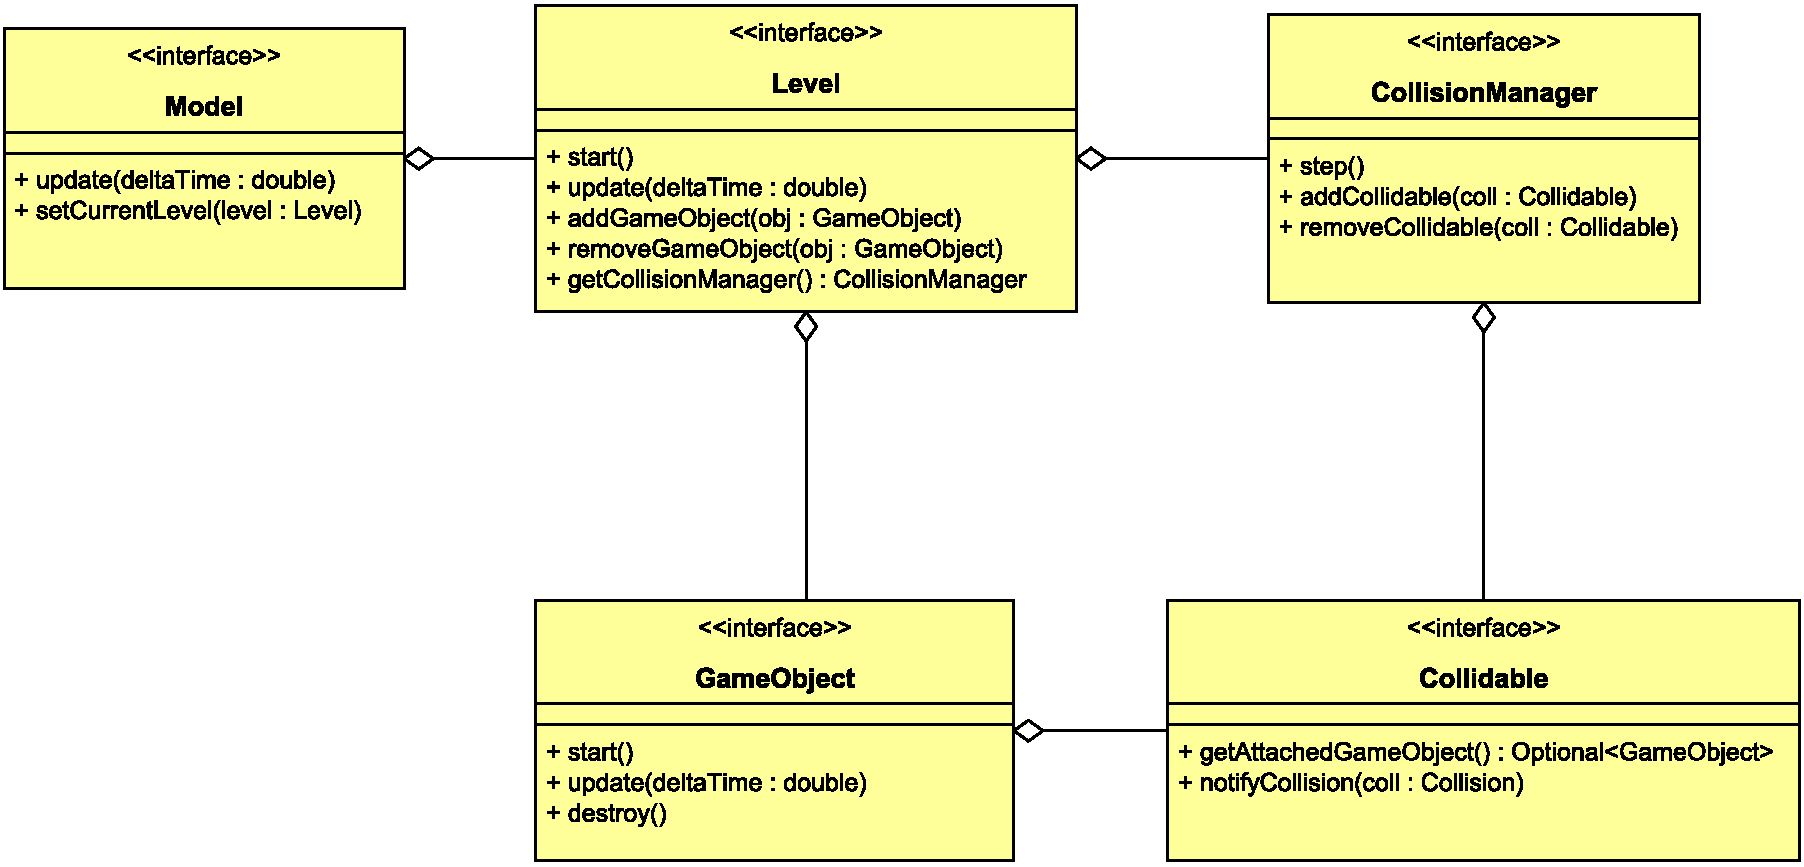
\includegraphics[width=\linewidth]{img/model}
\caption{Schema UML del modello del dominio.}
\label{img:model}
\end{figure}

\chapter{Design}

\section{Architettura}

Abbiamo scelto di utilizzare il pattern architetturale MVC per l'applicazione, in quanto uno dei pattern visti a lezione e perchè ci ha permesso di separare in maniera efficacie la logica di gioco dalle feature grafiche.
Nel nostro caso abbiamo creato un'interfaccia per ogni ambito in modo da semplificare le relazioni tra di esse.

\begin{figure}[H]
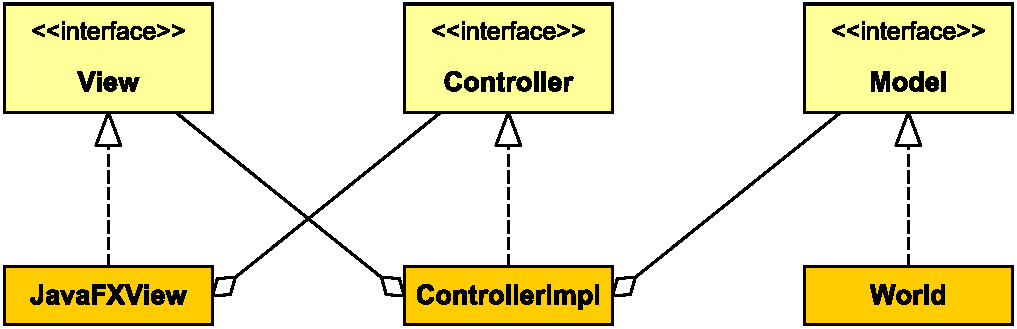
\includegraphics[width=\linewidth]{img/mvc}
\caption{Schema UML dell'architettura generale dell'applicazione e del pattern MVC.}
\label{img:mvc}
\end{figure}

In particolare l'interfaccia Model nasconde la logica in-game e la descrizione delle varie entità e di come interagiscono all'interno del Level.
Nella progettazione di questa componente abbiamo fatto in modo che fosse chiusa in se stessa.
Abbiamo dunque cercato di tenerla all'oscuro dell'esistenza di view e controller, rendendo quest'ultime responsabili di chiedere le informazioni necessarie.
Come mostrato nella \Cref{img:mvc} infatti, la componente Model non ha alcun riferimento alle altre componenti.

Nel Controller abbiamo inserito la gestione del flusso di utilizzo del software e dell'accesso ai dati persistenti (users e leaderboard).
Il suo compito principale è mantenere un'astrazione di GameSession (serie di livelli che termina all'esaurimento delle vite).
Ogni sessione apre per ogni livello un gestore del loop che aggiorna periodicamente il model, rappresentato dall'interfaccia GameLoop.

\begin{figure}[H]
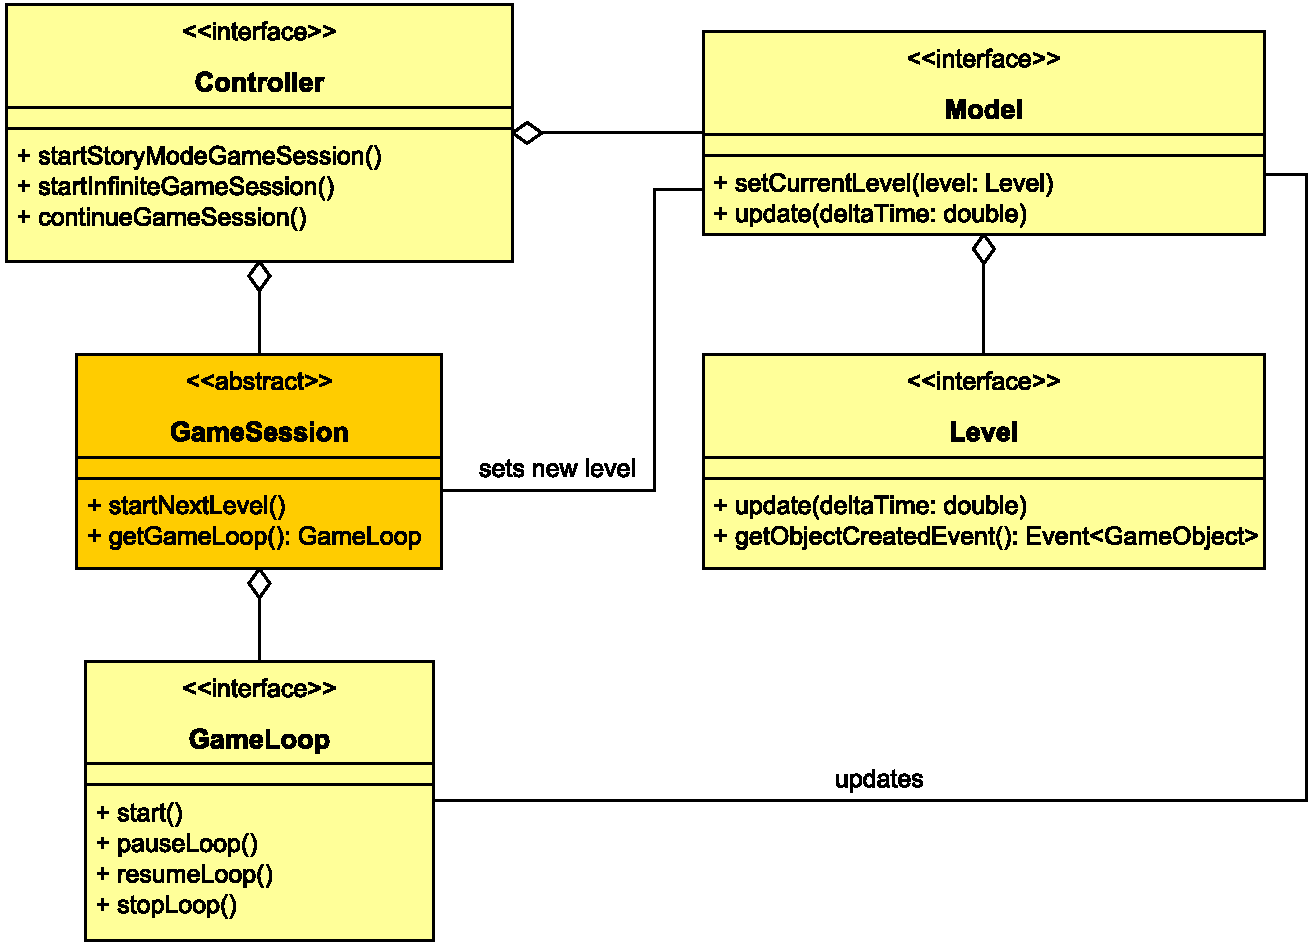
\includegraphics[width=\linewidth]{img/model_controller}
\caption{Schema UML che mostra l'interazione tra Controller e Model.}
\label{img:model_controller}
\end{figure}

Per quanto riguarda l'interazione con l'utente, la View si occupa della visualizzazione delle schermate dell'applicativo e nella fase di gioco del rendering del mondo.
Il metodo loadScene() modifica la schermata correntemente visualizzata, permettendo al controller di richiedere un cambio di scena.
Il rendering del mondo viene affidato al CanvasDrawer, componente della View il cui compito è la visualizzazione grafica effettiva del modello.
La richiesta di renderizzazione è effettuata dal GameLoop in seguito ad ogni fase di update del Model in modo da rispecchiare i cambiamenti avvenuti.

CanvasDrawer e Level svolgono dunque ruoli paralleli nei rispettivi ambiti dell'MVC, mantenendo aggiornati gli oggetti attivi e propagando le richieste del GameLoop su ognuno di essi.
Per questo motivo il CanvasDrawer svolge il ruolo di Observer nei confronti del Level, ottenendo così uno stato coerente tra parte logica e parte grafica.

\begin{figure}[H]
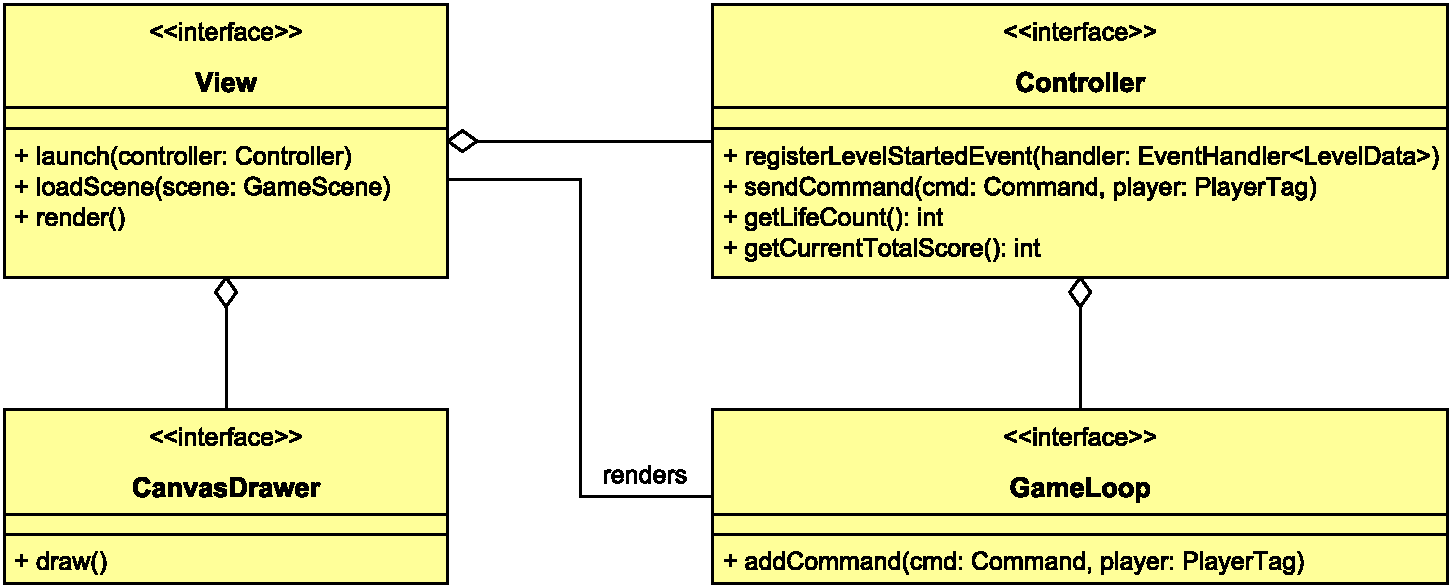
\includegraphics[width=\linewidth]{img/controller_view}
\caption{Schema UML che mostra l'interazione tra Controller e View.}
\label{img:controller_view}
\end{figure}

\section{Design dettagliato}

\subsection*{Samuele Burattini}

\subsubsection*{Shooting}

Per modellare l'azione di sparo di un proiettile ho identificato tre responsabiltà principali e ho deciso di affidarle a oggetti distinti per avere la massima flessibilità.

La responsabilità di creazione del proiettile è stata affidata all'interfaccia Shooter che descrive oggetti dotati di posizione e di un Supplier di Shot che gli permette di istanziare nuovi oggetti a partire appunto dalla posizione corrente dello Shooter stesso.

Allo ShooterComponent è affidato invece il compito di inviare le richieste fatte dal GameObject di cui fa parte lo Shooter e anche di mantenere quest'ultimo aggiornato alla posizione del GameObject.
Lo ShooterComponent utilizza lo Shooter via Strategy e può settare il suo stato a seconda se il GameObject ha richiesto di sparare o meno, ma è lo Shooter ad interpretare queste richieste in base alla propria politica interna.

Lo Shot invece gestisce il proprio comportamento in maniera indipendente.
Il metodo astratto handleCollision permette di modificare radicalmente il modo di comportarsi dello shot in relazione alla tipologia di oggetto colpito.

L'interazione tra Shooter e Shot è basata sul pattern Bridge in modo da legare direttamente l'interfaccia con la classe astratta e fare sì che ci sia compatibilità tra tutte le specializzazioni.
Ho fatto questa scelta proprio per rendere facile l'inserimento di armi con politiche di sparo diverso o di munizioni speciali e soprattutto per poterle combinare in maniera semplice dando la possibilità di un gameplay molto più vario.
Nella nostra versione del gioco ci siamo limitati ad implementare un solo shooter con due diversi tipi di HookShot sebbene la struttura supporti molte più variazioni.

\begin{figure}[H]
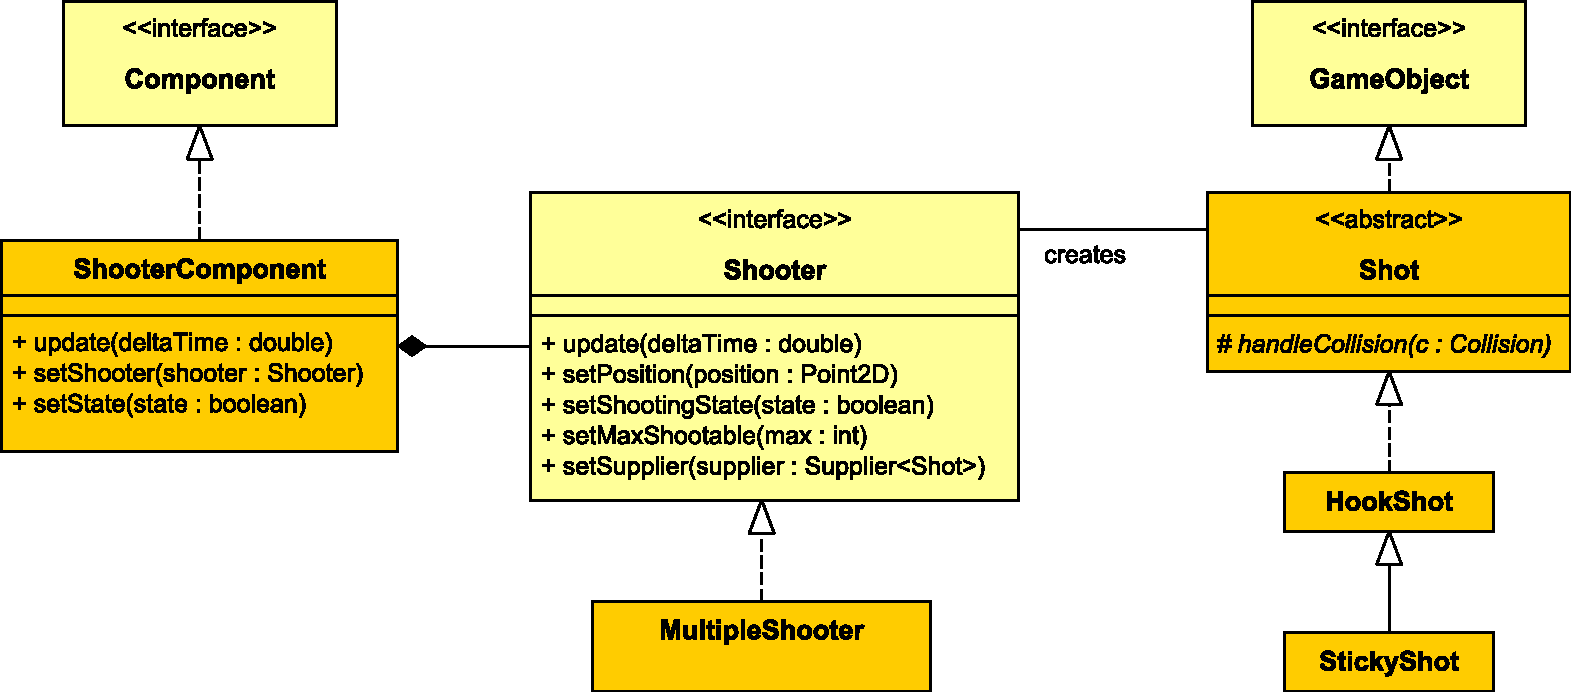
\includegraphics[width=\linewidth]{img/shooter}
\caption{Struttura del meccanismo di shooting in cui è visibile il pattern Bridge.}
\label{img:shooter}
\end{figure}

\subsection*{Nicholas Ciarafoni}

\subsection*{Francesco Dente}

\subsubsection*{Events}

Un elemento fondamentale della progettazione dell'applicazione è stata la modellazione del concetto di evento seguendo il pattern Observer.
In uno scenario così dinamico in cui lo stato del sistema cambia molto frequentemente, si intuisce chiaramente come la strategia di "polling" (interrogazione periodica) sia inefficacie.
Abbiamo dunque deciso di sfruttare questo pattern.

Il suo fulcro è l'interfaccia Event, che rappresenta un'avvenimento al quale uno o più listener (descritti dall'interfaccia EventHandler) possono interessarsi.
Ogni evento porta con se anche un tipo (T) relativo alle informazioni riguardanti l'avvenimento.

I metodi register() e unregister() permettono agli handler di iniziare o smettere di ascoltare l'evento stesso.
Dal momento della registrazione, ogni volta che l'evento viene innescato tutti i suoi osservatori vengono automaticamente notificati tramite il metodo handle().

La concretizzazione principale dell'interfaccia Event è EventSource, che contiene la logica per innescare l'evento e notificarne i gestori.
Ho deciso di non rendere disponibile il metodo trigger() tramite l'interfaccia per non dare la possibilità ad oggetti esterni al possessore dell'evento di innescarlo.
In questo modo solo la reale sorgente dell'evento ne ha la possibilità.

L'implementazione CompositeEvent rende invece possibile trattare più eventi "simili" come se fossero uno solo, seguendo appunto il pattern Composite.

Infine il NullEvent rappresenta un evento che, non potendo essere attivato, ignora semplicemente le richieste di register() e unregister().
La necessità di questa classe è dovuta alla presenza nel progetto di interfacce che richiedono la presenza di un certo evento.
Capita però in alcuni casi che certe implementazioni non siano realmente sorgenti per quel particolare evento.
In questo modo è possibile restituire comunque un oggetto compatibile con l'interfaccia Event anche se fasullo.

\begin{figure}[H]
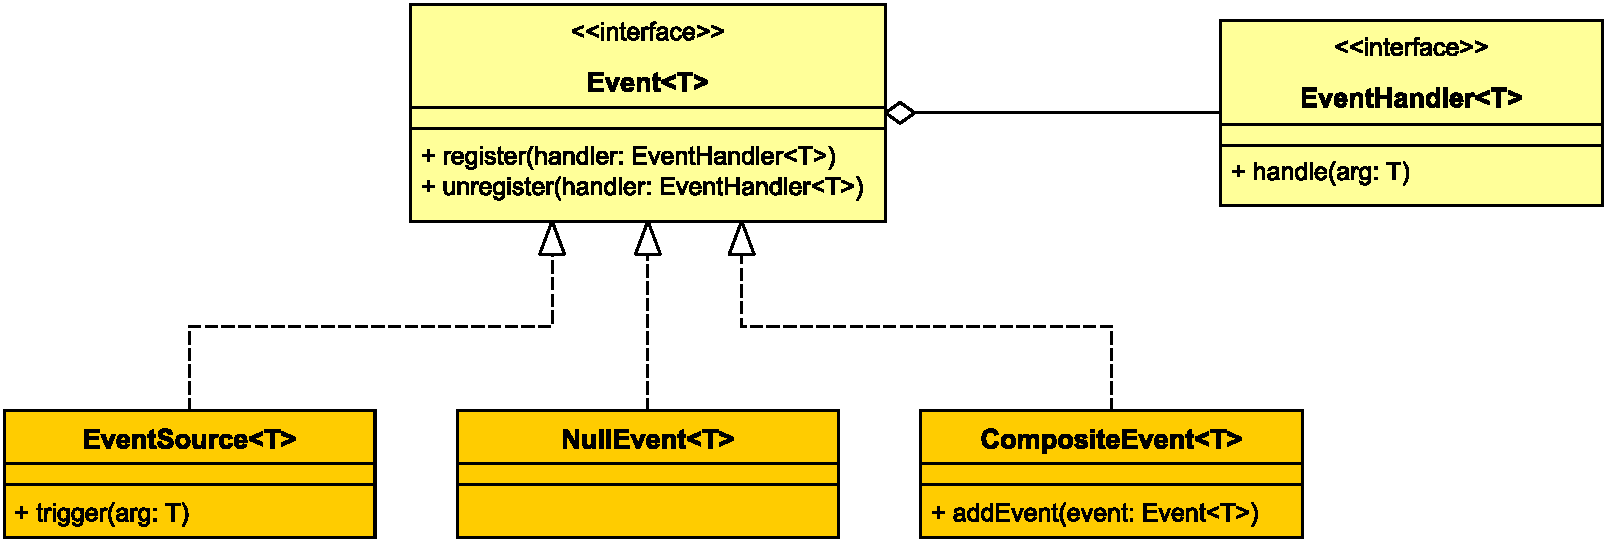
\includegraphics[width=\linewidth]{img/events}
\caption{Schema UML della struttura degli eventi.}
\label{img:events}
\end{figure}

\subsubsection*{Collisions}

Una parte di cui mi sono occupato è stata la rilevazione delle collisioni.
Nella scena sono infatti presenti entità che devono poter reagire non appena entrano in contatto con altri oggetti, ognuna secondo regole diverse.

Un'unità che ha la capacità di collidere viene rappresentata dall'interfaccia Collidable ed è dotata di una posizione e di una forma.
La gestione globale delle collisioni è invece affidata al CollisionManager che, venendo periodicamente richiamato dal Level, verifica quali coppie di Collidable sono in contatto in un determinato momento.
Ogni coppia viene quindi notificata tramite il metodo notifyCollision(), dove riceve informazioni riguardanti l'urto.
É compito del Collidable a questo punto informare chi è interessato tramite un evento.
Questo permette ai diversi GameObject che possiedono il Collidable di reagire in modo diverso alla collisione.

Sfruttando l'impalcatura fornita dai Component e il loro legame con i GameObject, ho pensato di implementare l'interfaccia Collidable tramite il CollisionComponent, permettendo facile accesso all'evento di collisione tramite l'interfaccia di GameObject.

\begin{figure}[H]
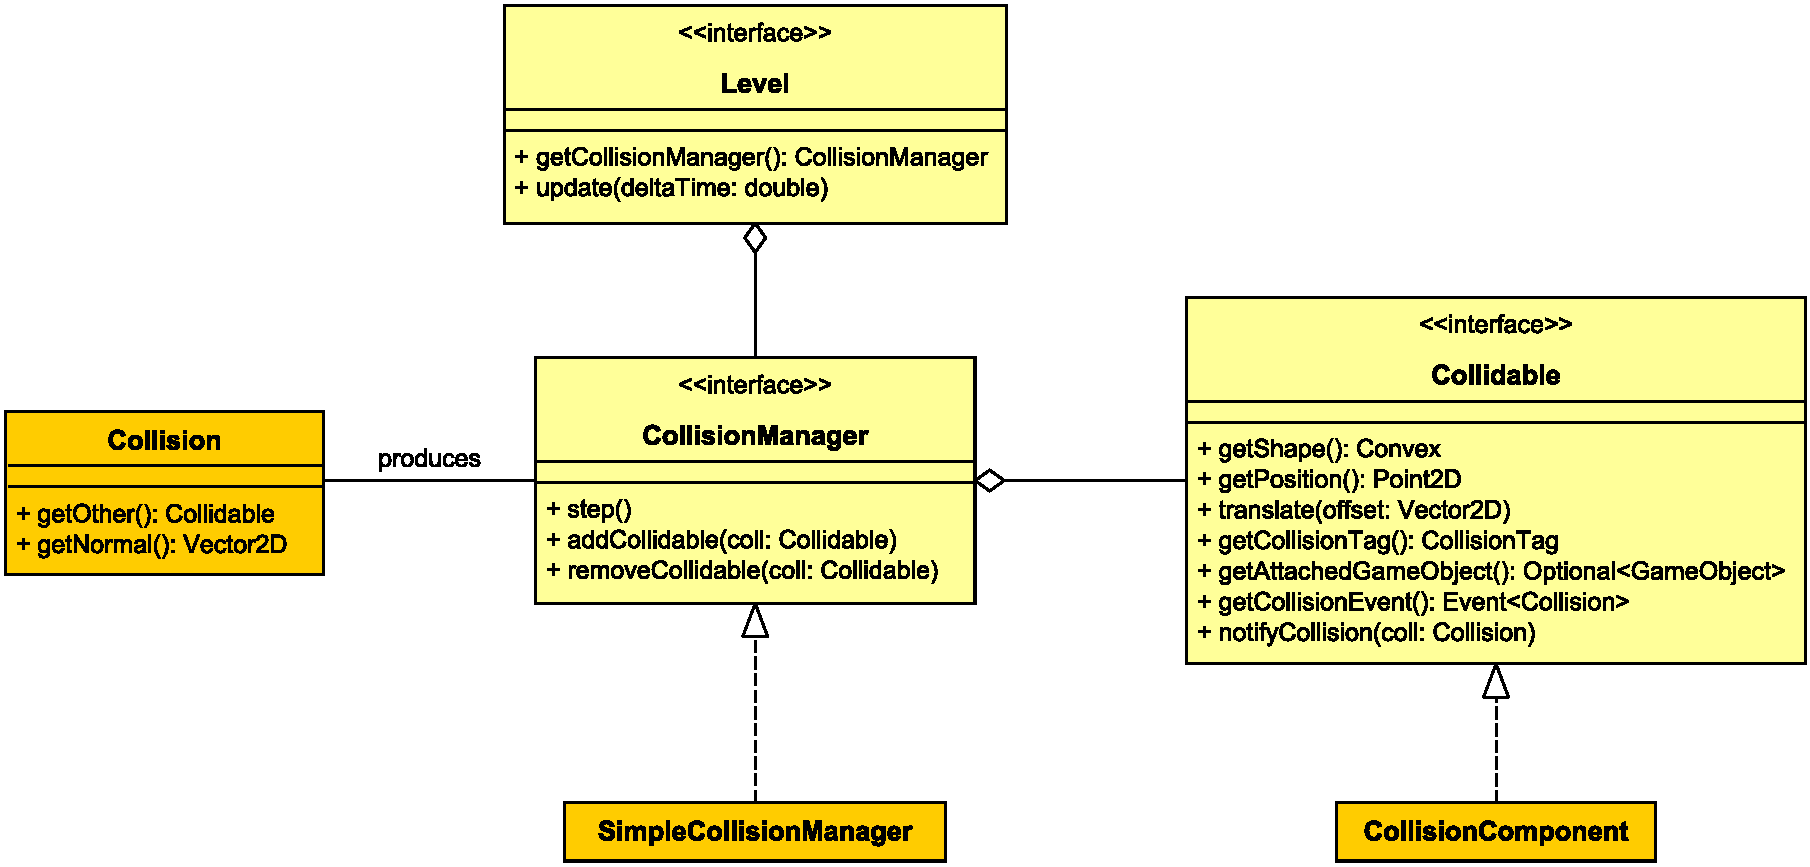
\includegraphics[width=\linewidth]{img/collisions}
\caption{Schema UML che descrive l'architettura per la gestione delle collisioni.}
\label{img:collisions}
\end{figure}

\subsubsection*{Rendering}

\begin{figure}[H]
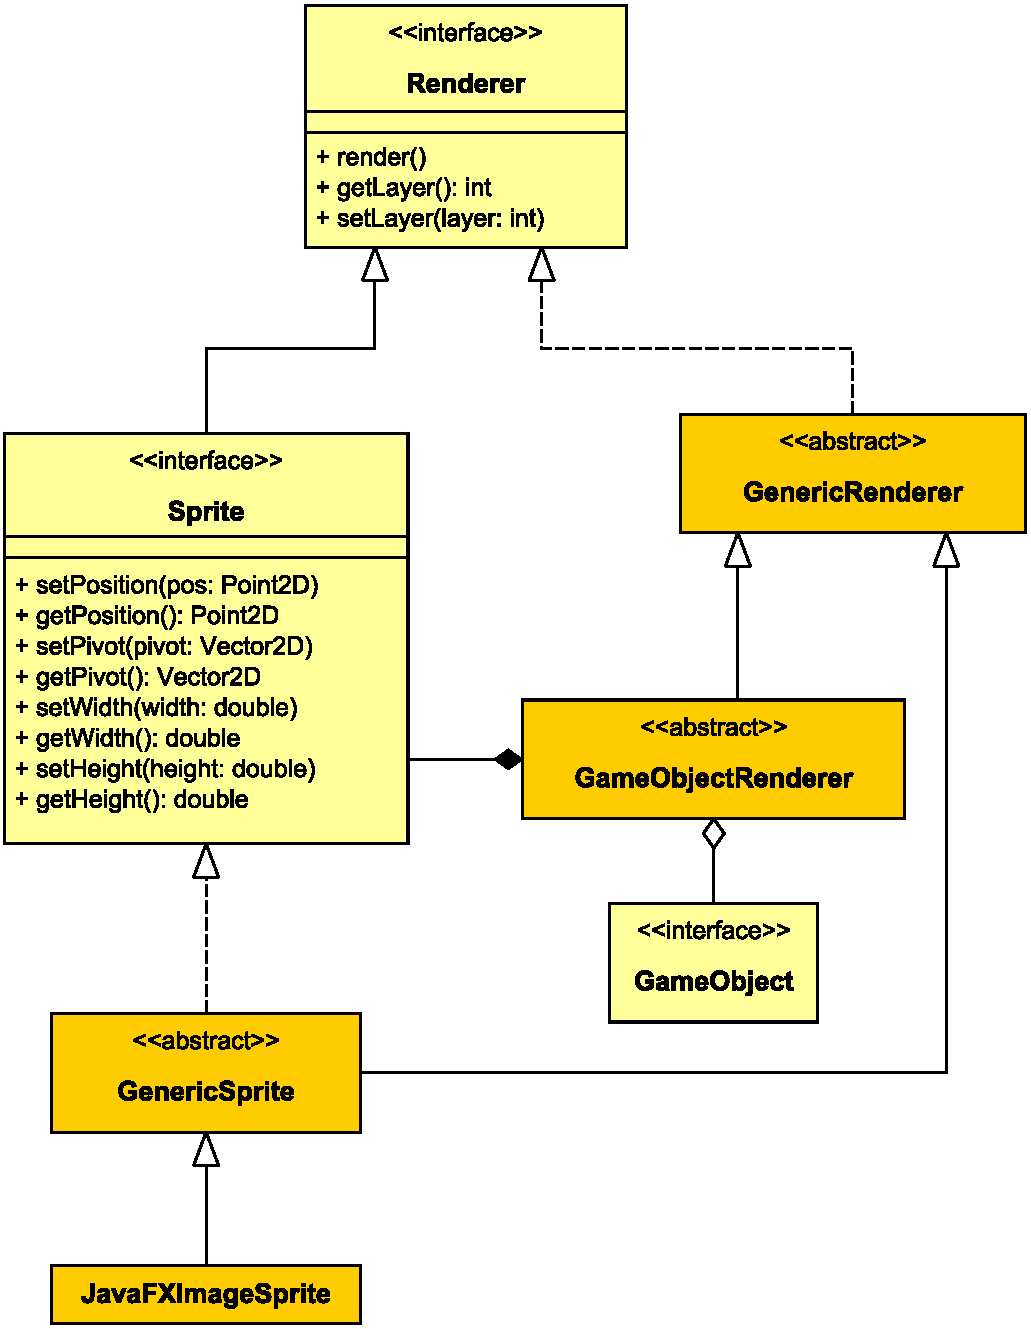
\includegraphics[width=\linewidth]{img/renderers}
\caption{Schema UML che mette in evidenza la gerarchia alla base della gestione del Rendering.}
\label{img:renderers}
\end{figure}

\begin{figure}[H]
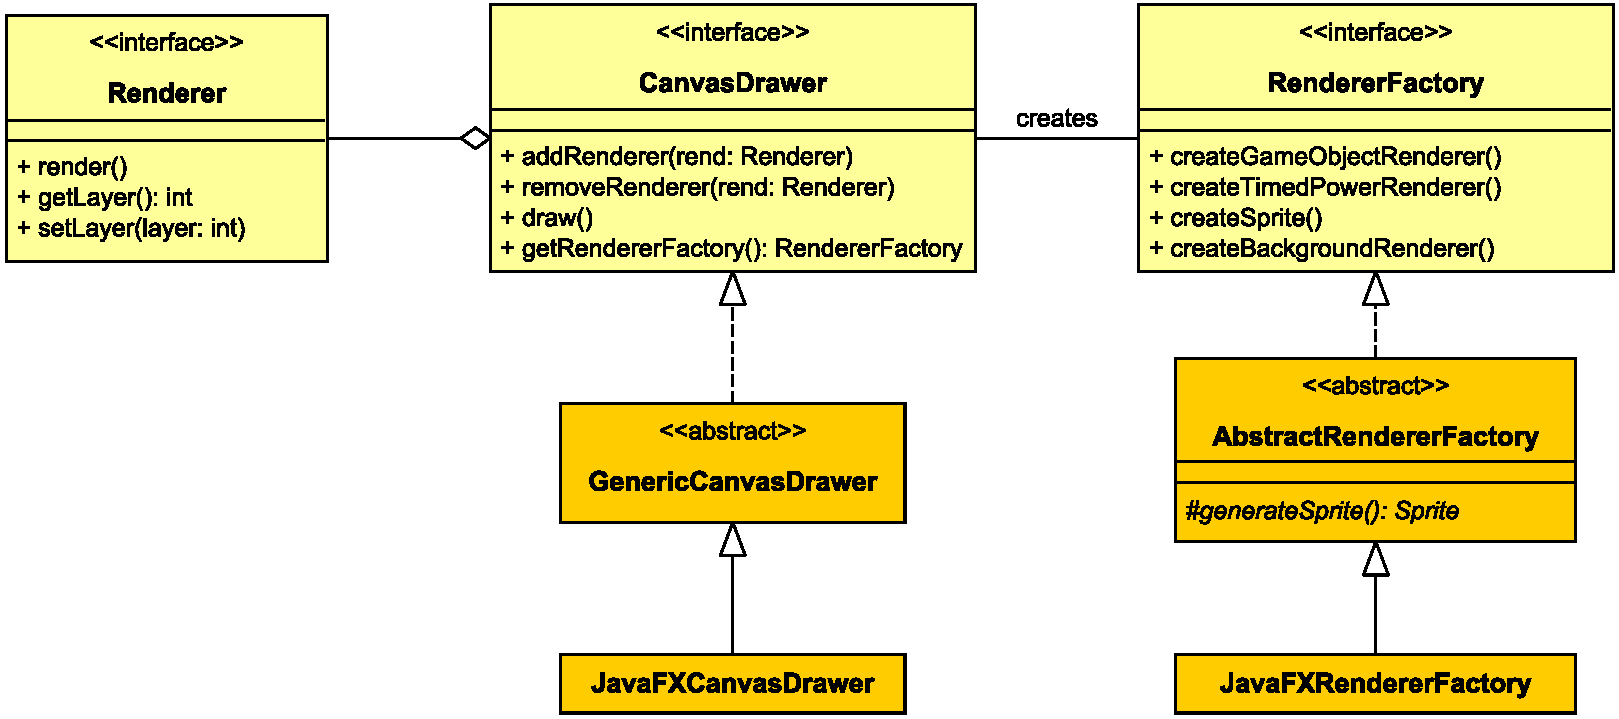
\includegraphics[width=\linewidth]{img/canvas_drawer}
\caption{Schema UML che mostra l'interazione tra Renderers e CanvasDrawer per mezzo della RendererFactory.}
\label{img:canvas_drawer}
\end{figure}

\subsubsection*{Decorators}

\begin{figure}[H]
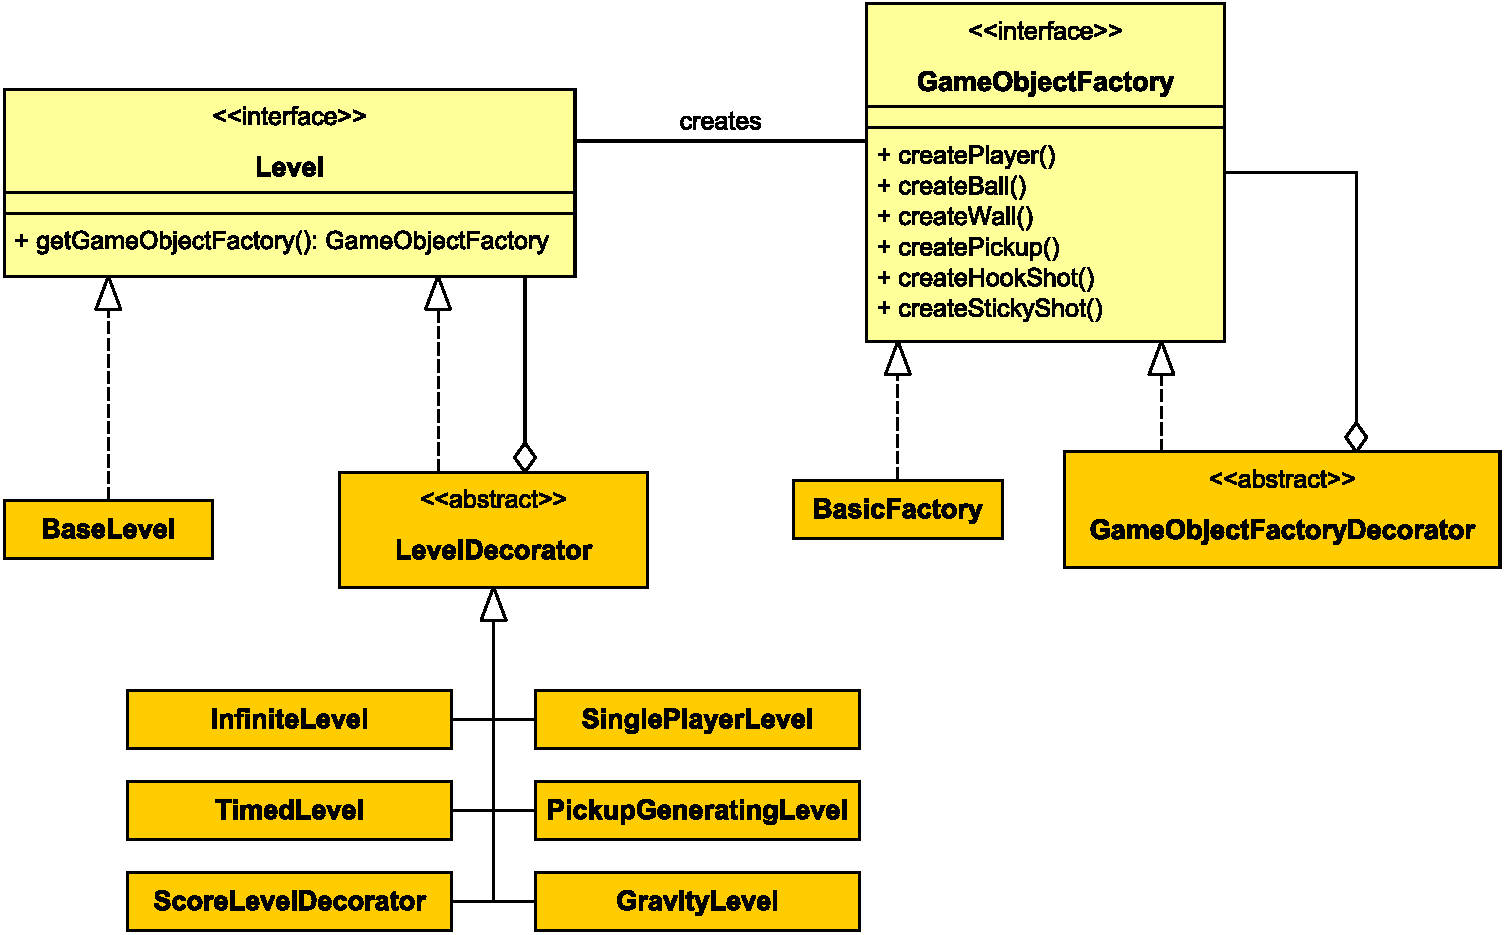
\includegraphics[width=\linewidth]{img/decorator}
\caption{Schema UML che mostra l'utilizzo del pattern Decorator per le interfacce Level e GameObjectFactory.}
\label{img:decorator}
\end{figure}

\subsection*{Lorenzo Menghini}

\subsection*{Francesca Tonetti}

\chapter{Sviluppo}

\section{Testing automatizzato}
Durante la fase iniziale dello sviluppo, nella quale ci siamo concentrati quasi esclusivamente sulla creazione del modello, abbiamo sentito la necessità di avere feedback sulla correttezza del lavoro svolto.
Abbiamo quindi pensato fosse un buon momento per iniziare a scrivere test automatizzati per le parti più critiche.
Per prima cosa abbiamo proceduto alla stesura di test per le collisioni (CollisionManager e Collidable), ritenuti di primaria importanza per via dell'uso della libreria dyn4j.
In seguito abbiamo optato per un test che verificasse che l'uso della Reflection per la ricerca di Component desse buoni risultati.
Successivamente ci siamo interessati alla correttezza dei meccanismi per l'input da parte dell'utente, testando in particolar modo la classe InputController.
Infine ci siamo dedicati a test per il funzionamento del Level e per l'aggiunta e rimozione di GameObject.

\section{Metodologia di lavoro}
Per sviluppare il progetto si è cercato di mantenere quanto possibile l'indipendenza delle parti assegnando aspetti distinti a ciascun membro del gruppo.
In un primo momento si è scelto di progettare nel dettaglio gli aspetti del dominio applicativo e di implementare quindi la parte Model dell'applicazione. 

Per una questione di coerenza interna la prima parte è stata svolta in collaborazione: una volta definite le interfacce principali per il Model, il Controller e la View si è passati alla definizione dei Component e lo sviluppo dei singoli GameObject nel dettaglio.
Ognuno ha quindi implementato un Component e un GameObject di cui essere responsabile.
Al fine di lavorare in parallelo ognuno ha inizialmente lavorato su un feature branch personale fino a che, una volta ottenuta una versione base funzionante dei singoli GameObject non sono stati tutti unificati su develop ed è iniziata la progettazione nel dettaglio del Controller e della View.
Degna di nota è stata l'aggiunta della GameSession che non era inizialmente prevista in fase di progettazione generale dell'applicazione, di cui però si è sentita l'esigenza per gestire in maniera più agevole tutto il flusso di gioco durante un'unica partita (fino ad esaurimento delle vite).
Parallelamente sul lato View ci si è concentrati sul rendering della scena di gioco e sulla creazione delle risorse grafiche.

Una volta ottenuta una versione "giocabile" dell'applicazione si sono iniziati a modellare i concetti di User, Leaderboard e le varie schermate di controllo in fxml, lavorando parallelamente sulla risoluzione di bug nel comportamento degli oggetti e dei poteri e sul generale del gioco.
L'ultima parte è stata principalmente dedicata alla stilizzazione grafica delle schermate e alla creazione dei livelli.

In generale la metodologia di sviluppo è stata più modulare che parallela e questo dovuto al fatto che la progettazione logica delle parti è stata abbastanza centralizzata e non affidata interamente ai singoli responsabili.
Questo, se anche in certi casi ha rallentato il gruppo, ha permesso di ottenere uno sviluppo molto coerente delle parti senza mai incontrare problemi nel processo di integrazione del codice sviluppato individualmente.

Per quanto in generale la tendenza sia stata quella di affidare la responsabilità di alcuni elementi ai singoli in alcune situazioni e specie in fase di bugfix ci sono stati piccoli interventi anche da parte di altri membri del gruppo.

In generale l'uso del DVCS è stato fatto seguendo i consigli ricevuti a lezione, cercando quindi di mantenere alcune feature isolate sui propri branch fino al loro effettivo completamento per non impattare sulla struttura principale.
Ciò è stato più facile nelle fasi iniziali di sviluppo del Model in quanto le parti erano più indipendenti, ma si è portata avanti la stessa filosofia dove possibile anche nello sviluppo complessivo dell'applicazione.

\section{Note di sviluppo}
Nello sviluppo dell'applicazione abbiamo cercato di utilizzare dove possibile gli elementi avanzati del linguaggio Java visti a lezione quali lambda expressions e Streams per avere un codice più facilmente comprensibile e semplice da scrivere.
Un caso degno di nota è quello dell'interfaccia funzionale oopang.commons.events.EventHandler, pilastro del meccanismo degli Observer presenti nel nostro progetto che è stata sempre utilizzata con l'utilizzo di lambda anche innestate.
Dove utile, in particolare per gli User e la Leaderboard, si è fatto uso di Optional e anche in tal caso si è preferito la creazione di lambda per programmare le azioni da eseguire sugli optional stessi.
In generale inoltre si è fatto uso di alcune delle interfacce funzionali fornite dal linguaggio Java quali Consumer e Supplier, molto utili per poter delegare delle operazioni senza creare veri e propri oggetti dedicati.

\chapter{Commenti finali}

\section{Autovalutazione e lavori futuri}

\end{document}
